\documentclass{article}
\usepackage[utf8]{inputenc}

\title{Graph Kernels and Support Vector Machines for Pattern Recognition}
\author{\textbf{Léo Andéol}\thanks{leo.andeol@gmail.com}\\ Master DAC, Sorbonne Université\\ Paris, France}
\date{May 2019}

\usepackage{natbib}
\usepackage{graphicx}
\usepackage{amsmath,amsthm,amssymb}
\usepackage{mathtools}
\usepackage{multicol}
\usepackage{url}
\usepackage{todonotes}
\usepackage{lipsum}

\DeclarePairedDelimiter{\abs}{\lvert}{\rvert}
\DeclarePairedDelimiter{\norm}{\lVert}{\rVert}

\let\vec\mathbf
\newcommand*{\C}{%
  \mathbb{C}%
}
\newcommand*{\R}{%
  \mathbb{R}%
}
\newcommand*{\Z}{%
  \mathbb{Z}%
}

\theoremstyle{definition}
\newtheorem{definition}{Definition}[section]

\begin{document}

\maketitle
\begin{abstract}
	\todo{ reecrire une fois rapport fini : Rajouter apport projet et facteur acceleration}\\
	Nowadays the world is turning to a new era where data is the most valuable resource, and we are working on algorithms to exploit those the best way possible. Most research is currently focused on the so-called "big data", huge quantities of data which are very sparse and of poor quality. However, there also exist structured databases of good quality, in the form of graphs, which is the one we will be studying. Graphs can be very useful in various fields, but is mostly known for its use in biology, as it can be used to represent proteins or other types of molecules.\\
	I chose to work on Support Vector Machines(cite qui/quand), a well known and powerful algorithm of machine learning. It is a perfect fit for studying graphs and learning to compare them because the algorithm allows through an elegant trick the use of several types of structured data.\\
	The goal of this project is to implement a working algorithm and its improvements, test it on different types of data and try to improve it.
\end{abstract}

\newpage

\tableofcontents

\newpage

\section{Introduction}
 \todo{introduction générale plus étendue : 1 et 1/2 page :donner un aperçu/résumé du rapport : un paragraphe par élément - ECRIRE A LA FIN}
 \lipsum[1-8]
\section{Methodology}
 \todo{Est-ce que c'est la bonne expression en anglais ?}
\subsection{Background}
sous section 1 : background : graphe, svm, noyaux, donner toutes les définitions.
\subsubsection{Graphs}
\todo{Reference pour graphes}
A graph\cite{graph_wiki} is a type of mathematical structure that represents the connection between object. It is thus composed of vertices (or nodes) and edges. Vertices represent objects and are usually depicted as circles or spheres whereas edges link pairs or vertices. 
\begin{definition}
	A graph is an ordered pair $G=(V,E)$ where :
	\begin{itemize}
		\item $V$ is a set of nodes
		\item $E \subseteq {(u,v) | (u,v) \in V^2}$
	\end{itemize}
\end{definition}
\begin{figure}[!htb]
\begin{multicols}{2}
    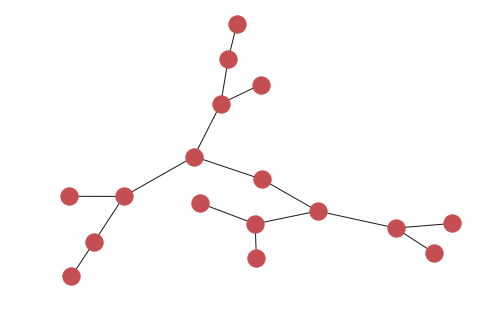
\includegraphics[width=\linewidth]{data/graphs/big_graph_no_label.png}\par
    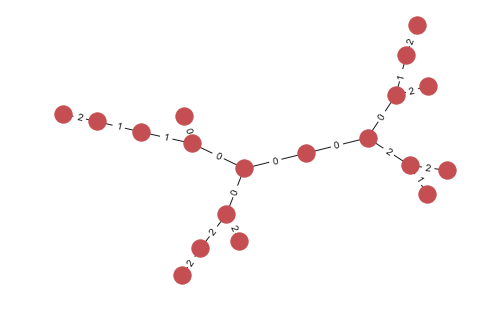
\includegraphics[width=\linewidth]{data/graphs/big_graph_label.png}\par
\end{multicols}
\caption{Two "tree" graphs, resp. unlabeled and labeled}
\end{figure}
The edges of the graph can be weighted and can be either oriented or not. We will be focusing on undirected unweighted graphs, thus we have :
\begin{definition}
	$\forall (u,v) \in E \implies (v,u)\in E$
\end{definition}
Both vertices and edges can have labels, which can take various forms : they can be elements of a finite or infinite set (such as integers but also strings), or even continuous (such as $\in \R$).
Graphs were first used in their modern form to represent the problem of Seven Bridges of Königsberg (cite), and have been ever since used to represent maps, and thus path-finding algorithms were developed. Graphs can also be used, with labels, to represent different type of molecules and interactions between them.(parler aussi des réseaux ? des problemes de flots etc ?)\\
During this project, we will focus on undirected graphs which can have any type of labels on their edges only (if it is only on their nodes, the complementary graph can be studied).\\
We will be comparing graphs in order to find similarities between them, and classify them in different groups. It has been shown(cite) that it can be used effectively on proteins and (?).
\subsubsection{Support Vector Machines}
Support Vector Machines (SVM) are a type of machine learning algorithms discovered in the early 90s(cite). It was originally a classification algorithm however it has been expanded since to regression and clustering too. It is especially powerful and widely used for two main reasons :
\paragraph{Margin and support vectors}
The Support Vector Machines were based on the model of the Perceptron (cite), another classification algorithm that tried to find an hyperplane that discriminates the two sets.\\
The main issue with the Perceptron is that it had no formal guarantee to find an optimal hyperplane, and more often than not would not find it. Moreover, if the data weren't linearly separable, the algorithm would not converge.\\
In order to tackle theses issues, the SVM offered three fixes. \\
First, they added a margin in the loss function in order to not only classify well the data samples, but also with the maximum certainty, i.e. as far from the decision boundary as possible.\\
\begin{equation}
    L(y,x,w) = \max(0,-y*x \cdot w) \implies L(y,x,w) = \max(0,1-y*x\cdot w)
\end{equation}
Then, seeing this solution wasn't enough, as there was still an infinity of possible solutions, it was proven that the margin between points and the decision boundary was inversely proportional to the norm of the weights.\\
\begin{equation}
\gamma = \frac{y_{i}(x_{i} \cdot w + w_{0})}{\norm{w}}
\end{equation}
These two fixes gave us the first version the SVM, the hard-margin SVM :\\ 
\begin{equation}
    \min \frac{1}{2}\norm{w}^{2} \quad
\textup{s.t.}\quad y_{i}(x_{i} \cdot w + w_{0}) \geq 1 \quad \forall i \in \{1..n\}
\end{equation}
However, if the data weren't linearly separable the algorithm wouldn't be optimizable since the quadratic programming problem requires all points to be correctly classified. Then, a new term $\xi$ was introduced as an error tolerance, as well as a factor $C$ that would determine the balance between error tolerance and weights minimization.\\
\begin{equation}
\begin{array}{ll@{}ll}
\text{min}  & \frac{1}{2}\norm{w}^{2}+C\sum\limits_{i=1}^{n}\xi_{i} &\\
\text{s.t.}& \forall i \in \{1..n\} & y_{i}(x_{i} \cdot w + w_{0}) \geq 1-\xi_{i}
\end{array}
\end{equation}
\subsubsection{Kernels}
In its dual form, the SVM problem only requires a dot product between the sample vectors. Then, we can use a nonlinear transformation $\phi(x)$ to replace the dot-product $\vec{x_i} \cdot \vec{x_j}$ by $\phi(\vec{x_{i}})\cdot\phi(\vec{x}_{j})$ , effectively augmenting the dimensions of our vectors and thus the expressiveness of our model by enhancing the separability of the data. However, for complex transformations, such as in infinite dimensions, the function $\phi$ isn't defined. But it was found(cite) that the standard dot product can be replaced by another function as long as it is a bilinear positive semi definite form. 
\begin{equation}
    \sum\limits_{i=1}^{n}\sum\limits_{i=1}^{n}K(\vec{x_{i}},\vec{x_{j}})c_{i}c_{j} \geq 0 \qquad \forall i \in \{1..n\} \quad c_i \in \R
\end{equation}
Thus, the dot product can be replaced by a function $K(x_1,x_2)$ which will indirectly (?) transform the data in larger dimensions, even infinite with the Gaussian kernel(cite) and return the dot product of those transformations, while remaining computable in all cases. This replacement is usually called the "Kernel Trick".\\
Ever since the foundation of SVMs, the kernel trick became a big focus of the machine learning community as it naturally fits in the algorithm and allows supervised learning on very complex data, and enjoying greater accuracy than most algorithms.
\subsection{State of the Art}
sous section 2 : state of the art : graph kernels et acceleration des random walk, donner les complexité, donner des exemples, discuter avantages et inconvenients chacun
\subsubsection{Introduction}
In this chapter we will discuss the advance of research on graph kernels. Graph kernels have been studied since Support Vector Machines started getting popular(cite). Since then, a lot of progress has been made, and several types of kernels have been discovered, such as random walk and graphlet kernels, the two we will be stuyding, but not the only ones. There are also graph kernels that use spanning trees, and several others that are unfortunately usually not semi definite(cite nino).
\url{R-convolution kernels, rational kernels}\\
\url{source: https://publikationen.uni-tuebingen.de/xmlui/bitstream/handle/10900/49731/pdf/thesis_all.pdf?sequence=1&isAllowed=y}
\subsubsection{Graphlets}
A graphlet(cite) is a subgraph of 3,4 or 5 nodes taken from a much larger graph. The idea of a graphlet kernel is to count all types of graphlets that appear in a graph, and use that count to compare to another graph.\\
insert list of graphlets
\subsubsection{Random walks}
The state of the art of this type of kernel is mainly defined in Graph Kernels(cite) although there have been several other developments recently (cite). Random walks are a type of rather intuitive algorithms : as its name says, it randomly walks through a graph for a certain time, and we can use these walks to compare graphs as it has been shown(cite). Actually, we will walk through all possible paths in the graph we will compare using a simple trick : by making the adjacency matrix stochastic, we can use it as a markov chain. Moreover, it has also been shown(cite) that performing a walk on two separate graphs at the same time is the same as performing a walk on the product graph. The product graph is in computer science terms the Cartesian product of the two graphs, taking all possible combinations of edges and nodes, but mathematically, the adjacency matrix of a such graph is the result of the Kronecker product of the two graphs(cite) (expliquer?) :
\begin{equation}
    W_{\times}=A \otimes A_{2}
\end{equation}
\subsubsection{Kernel definition}

\subsubsection{Sylvester Equation}
A Sylvester equation, also sometimes called Lyapunov equation (a generalized version of it) is a matrix equation of the following shape :
\begin{equation}
    AX+XB=C
\end{equation}
However, there also exist a discrete-time version of it :
\begin{equation}
    AXB+C=X
\end{equation}
TODO solvable how, what efficiency\\

\subsubsection{Conjugate Gradient Method}
Note : Preconditioner random vector : $x \cdot x^{T}$ fonctionne bien\\
The Conjugate Gradient Method is an optimization algorithm used to find approximate solutions of linear systems that have a positive semi definite matrix. As its name suggests, it is a gradient based (usually) iterative algorithm. The Main idea is 
\subsubsection{Fixed-Point Iterations}
si lambda trop proche de l'inverse de la valeur propre peut etre tres lent à converger quand la matrice d'adjacence est très dense\\
Fixed point consists in ....\\
proof that $\lambda<|\xi|^{-1}$
\begin{proof}
  Let $x_0=p_\times$ and $t>>0$
  \begin{align*}
      x_{t+1}-x_t &= p_\times+\lambda W_{\times} x_t - x_t &\\
      &= p_{\times}+(\lambda W_{\times} - 1)(p_{\times}+\lambda W_{\times} x_{t-1})\\
      &= p_{\times} - p_{\times} + \lambda W_{\times}p_{\times} + (\lambda W_{\times})^2 x_{t-1} - \lambda W_{\times} x_{t-1}\\
      &= \lambda W_{\times}(p_{\times}-x_{t-1}+\lambda W_{\times} x_{t-1}) \\
      &= \lambda W_{\times}(p_{\times}-\lambda W_{\times} x_{t-2} - p_{\times} + \lambda W_{\times}(\lambda W_{\times} x_{t-2} +p_{\times}) \\
      &= \lambda W_{\times} ( \lambda W_{\times} (\lambda W_{\times} x_{t-2}+p_{\times}-x_{t-2})) \\
      &= (\lambda W_{\times})^2(\lambda W_{\times} x_{t-2}+p_{\times} - x_{t-2}) & \\
      \text{We find a pattern}\\
      \implies x_{t+1}-x_t &= (\lambda W_{\times})^t (\lambda W_{\times} x_0 + p_{\times} - x_0) & \\
      \text{And because } x_0 = p_{\times}\\
      &= (\lambda W_{\times})^{t+1} p_{\times}\\
      \text{Which decreases only when}\\
      \xi_1 < 1\\
      \text{The largest magnitude eigenvalue of} \lambda W_{\times}\\
      \implies \lambda < |\xi_1|^{-1}
      && \qedhere
  \end{align*}
  Rapidité de la convergence : géométrique avec un ratio $\lambda$1/$\lambda$2???
\end{proof}

\subsection{Contributions}
en anglais ça donne ?



\section{Experiments}
experiences : détailler db, tests, méthodes, les parametres, construction label, donner tableaux, resultats, teps de calculs, précision, discuter tout cela
\subsubsection{Spectral Decompostion}
can't inverse Left eigenvectors : 
\url{https://arxiv.org/pdf/1708.00064.pdf}
\subsubsection{Nearest Kronecker Product}
\url{https://www.sciencedirect.com/science/article/pii/S0377042700003939?via%3Dihub}
	\url{https://www.imageclef.org/system/files/CLEF2016_Kronecker_Decomposition.pdf}
	\url{http://dx.doi.org/10.1007/978-94-015-8196-7_17}
	\url{https://mathematica.stackexchange.com/questions/91651/nearest-kronecker-product}
	
\subsection{Implementation}
\subsubsection{Graph Database}
The first step was to create a graph database generator that we would use to test our algorithms on simple cases with expectable behaviour. I have chosen to focus on 3 types of graphs (todo expand) : ring, star and tree graphs.\\
The graph generator can create graphs that are either labelled or unlabelled. As for labelled ones, it will simply assign to all edges a random integer between 1 and the given limit during the creation of the database.
\begin{figure}[!htb]
\begin{multicols}{4}
    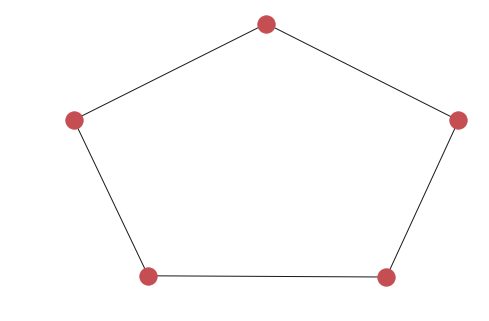
\includegraphics[width=\linewidth]{data/generated-graphs/ring_base.png}\par
    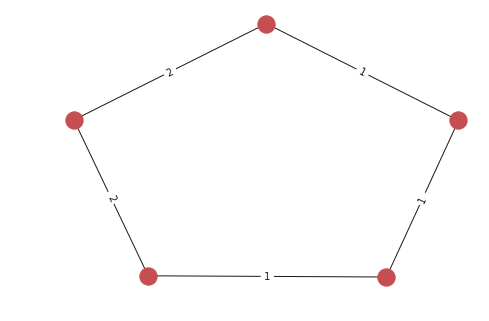
\includegraphics[width=\linewidth]{data/generated-graphs/ring_labels.png}\par
    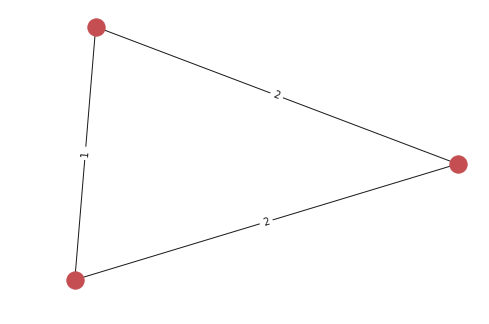
\includegraphics[width=\linewidth]{data/generated-graphs/ring_altered_struct.png}\par
    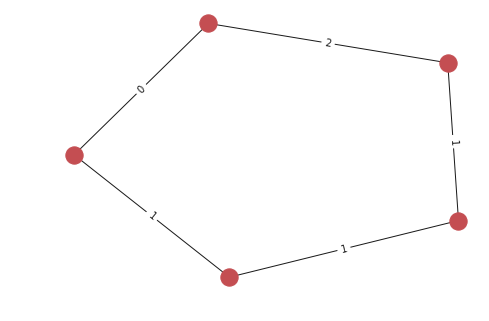
\includegraphics[width=\linewidth]{data/generated-graphs/ring_altered_labels.png}\par
\end{multicols}
\caption{Ring graphs, resp. unlabelled, labelled, altered structured, altered labels}
\end{figure}
Moreover, the database generator will also alter all generated graphs both structurally and on labels. Concerning labels, some edges are picked in the graph following a limit given by the user and the new label values of those edges are randomly generated in the same set as the original ones.
\begin{figure}[!htb]
\begin{multicols}{4}
    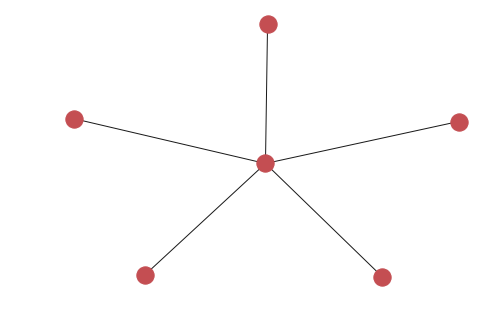
\includegraphics[width=\linewidth]{data/generated-graphs/star_base.png}\par
    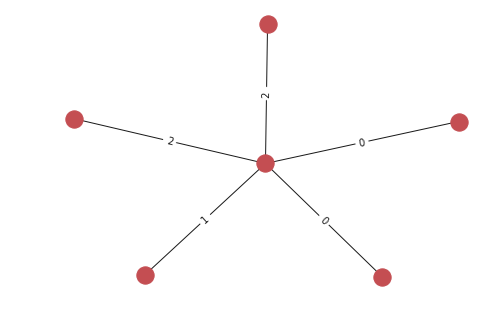
\includegraphics[width=\linewidth]{data/generated-graphs/star_labels.png}\par
    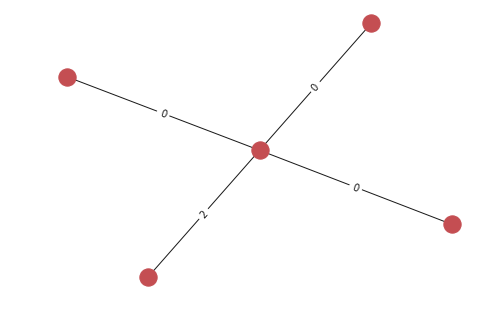
\includegraphics[width=\linewidth]{data/generated-graphs/star_altered_struct.png}\par
    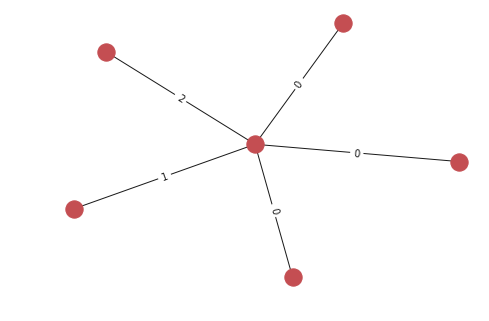
\includegraphics[width=\linewidth]{data/generated-graphs/star_altered_labels.png}\par
\end{multicols}
\caption{Star graphs, resp. unlabelled, labelled, altered structured, altered labels}
\end{figure}
Finally, the structure of generated graphs will be altered depending on their type, but will always keep the same set of labels (except for new edges).
\begin{enumerate}
    \item Ring graphs are simply regenerated slightly longer or shorter randomly.
    \item Star graphs are also regenerated either with more or less nodes, randomly.
    \item Tree graphs are either expanded by adding randomly leaves anywhere in the graph, or reduced by randomly removing leaves.
\end{enumerate}
\begin{figure}[!htb]
\begin{multicols}{4}
    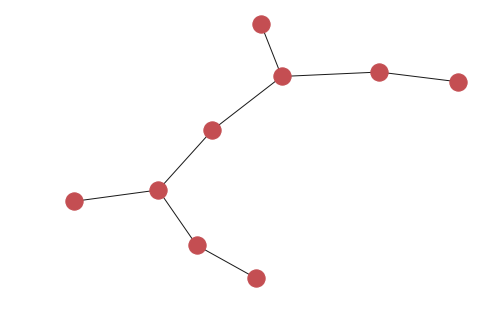
\includegraphics[width=\linewidth]{data/generated-graphs/tree_base.png}\par
    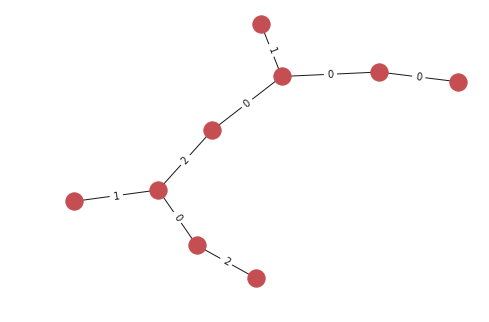
\includegraphics[width=\linewidth]{data/generated-graphs/tree_labels.png}\par
    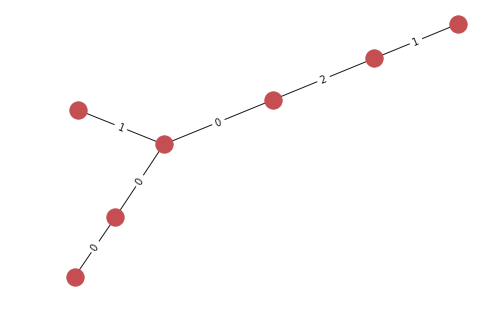
\includegraphics[width=\linewidth]{data/generated-graphs/tree_altered_struct.png}\par
    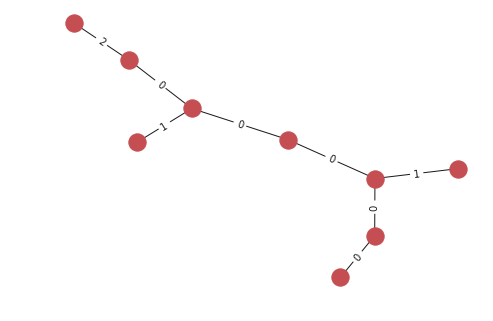
\includegraphics[width=\linewidth]{data/generated-graphs/tree_altered_labels.png}\par
\end{multicols}
\caption{Tree graphs, resp. unlabelled, labelled, altered structured, altered labels}
\end{figure}
After having generated the whole database, graphs will be transformed to adjacency matrices since we will only be handling graphs under this form. For unlabelled graphs, it simply returns the adjacency matrix (expliquer ce que c'est ?) and for labelled graphs it returns an array of adjacency graphs, only considering the partial graph of the edges of a particular label at a time.
\subsubsection{Kernels}

\subsection{Test of the random walk kernel}
\subsubsection{Accuracy comparison between labelled and unlabelled graphs}
Même score, car donne même matrice ???
\begin{table}[!htb]
\begin{center}
\begin{tabular}{|l|l|l|}
    \hline
    & Unlabelled & Labelled \\
    \hline
    Accuracy & ? & ? \\
    \hline
    Time & ? & ? \\
    \hline
\end{tabular}
\end{center}
\caption {Time and Accuracy of learning resp. for unlabelled and labelled graphs} \label{tab:lab_vs_nolab} 
\end{table}

\subsubsection{Efficiency of alternate methods}
\begin{table}[!htb]
\begin{center}
\begin{tabular}{|p{15mm}|p{15mm}|p{15mm}|p{15mm}|p{15mm}|p{15mm}|p{15mm}|p{15mm}|}
    \hline
    & Raw\newline kernel & Inverse\newline Kernel & Sylvester\newline Equation & Conjugate\newline Gradients & Fixed\newline points & Spectral\newline Decomp. & Nearest\newline Kronecker Product \\
    \hline
    Accuracy & 67\% & 67\% & ? & 67\% & 67\% & ? & ? \\
    \hline
    Time & 18.40s  & 5.72 & ? & 7.62s & 5.94s & ? & ? \\
    \hline
\end{tabular}
\end{center}
\caption {Time and Accuracy of learning for the raw kernel and other methods} \label{tab:kernel_comparison} 
\end{table}
\subsubsection{Experiments on a biology dataset}
\url{https://ls11-www.cs.tu-dortmund.de/staff/morris/graphkerneldatasets} 
\url{http://members.cbio.mines-paristech.fr/~nshervashidze/code/}
enzymes
\subsection{Improvements}

\section{Conclusion and Future Work}
experiences : détailler db, tests, méthodes, les parametres, construction label, donner tableaux, resultats, teps de calculs, précision, discuter tout cela
section 4 : 1 page ou page et demi : conclusion et discussion


\appendix
\section{Appendix}
\section{Annex 1}

\section{Acknowledgements}
This work was done during the first year of my master.

\listoffigures
\listoftables
bibliographie et index

\bibliographystyle{ieeetr}
\bibliography{references}
\end{document}
